\documentclass{article}
\usepackage[utf8]{inputenc}
\usepackage{kotex}
\usepackage{url}
\usepackage{cancel}
\usepackage{xspace}
\usepackage{graphicx}
\usepackage{multicol}
\usepackage{multirow}
\usepackage{subfig}
\usepackage{amsmath}
\usepackage{amssymb}
\usepackage[a4paper, width=186mm, top=18mm, bottom=18mm, includeheadfoot]{geometry}
\usepackage{booktabs}
\usepackage{array}
\usepackage{verbatim}
\usepackage{capt-of}
\usepackage{natbib}
\usepackage{booktabs}
\usepackage{float}
\usepackage{pdflscape}
\usepackage{mathtools}
\usepackage[usenames, dvipsnames]{xcolor}
\usepackage{afterpage}
\usepackage{pgf}
\usepackage{tikz}
\usepackage{dirtree}
\usepackage[style=american]{csquotes}
\usepackage{amsfonts}
\usepackage{tikz}
\usepackage{tkz-graph}
\usepackage{indentfirst}
\usetikzlibrary{arrows,decorations.pathmorphing,automata,positioning,backgrounds,fit,shapes.symbols,chains,intersections}


\newtheorem{definition}{정의}[section]
\newtheorem{theorem}{Theorem}[section]
\newtheorem{lemma}{Lemma}
\newtheorem{proof}{Proof} [section]


\usepackage[toc, page, title, titletoc, header]{appendix}
\usepackage{marginnote}
\usepackage{tablefootnote}


\renewcommand\appendixname{첨\부 }
\renewcommand\appendixpagename{첨\부}
\renewcommand\appendixtocname{첨\부}
\renewcommand\abstractname{적요}

\usepackage{perpage} %the perpage package
\MakePerPage{footnote} %the perpage package command

\usetikzlibrary{shapes.geometric}%
\usepackage{color}

%\usepackage[pages=some, placement=top]{background}

\usepackage{eso-pic}
\usepackage[final]{pdfpages}

%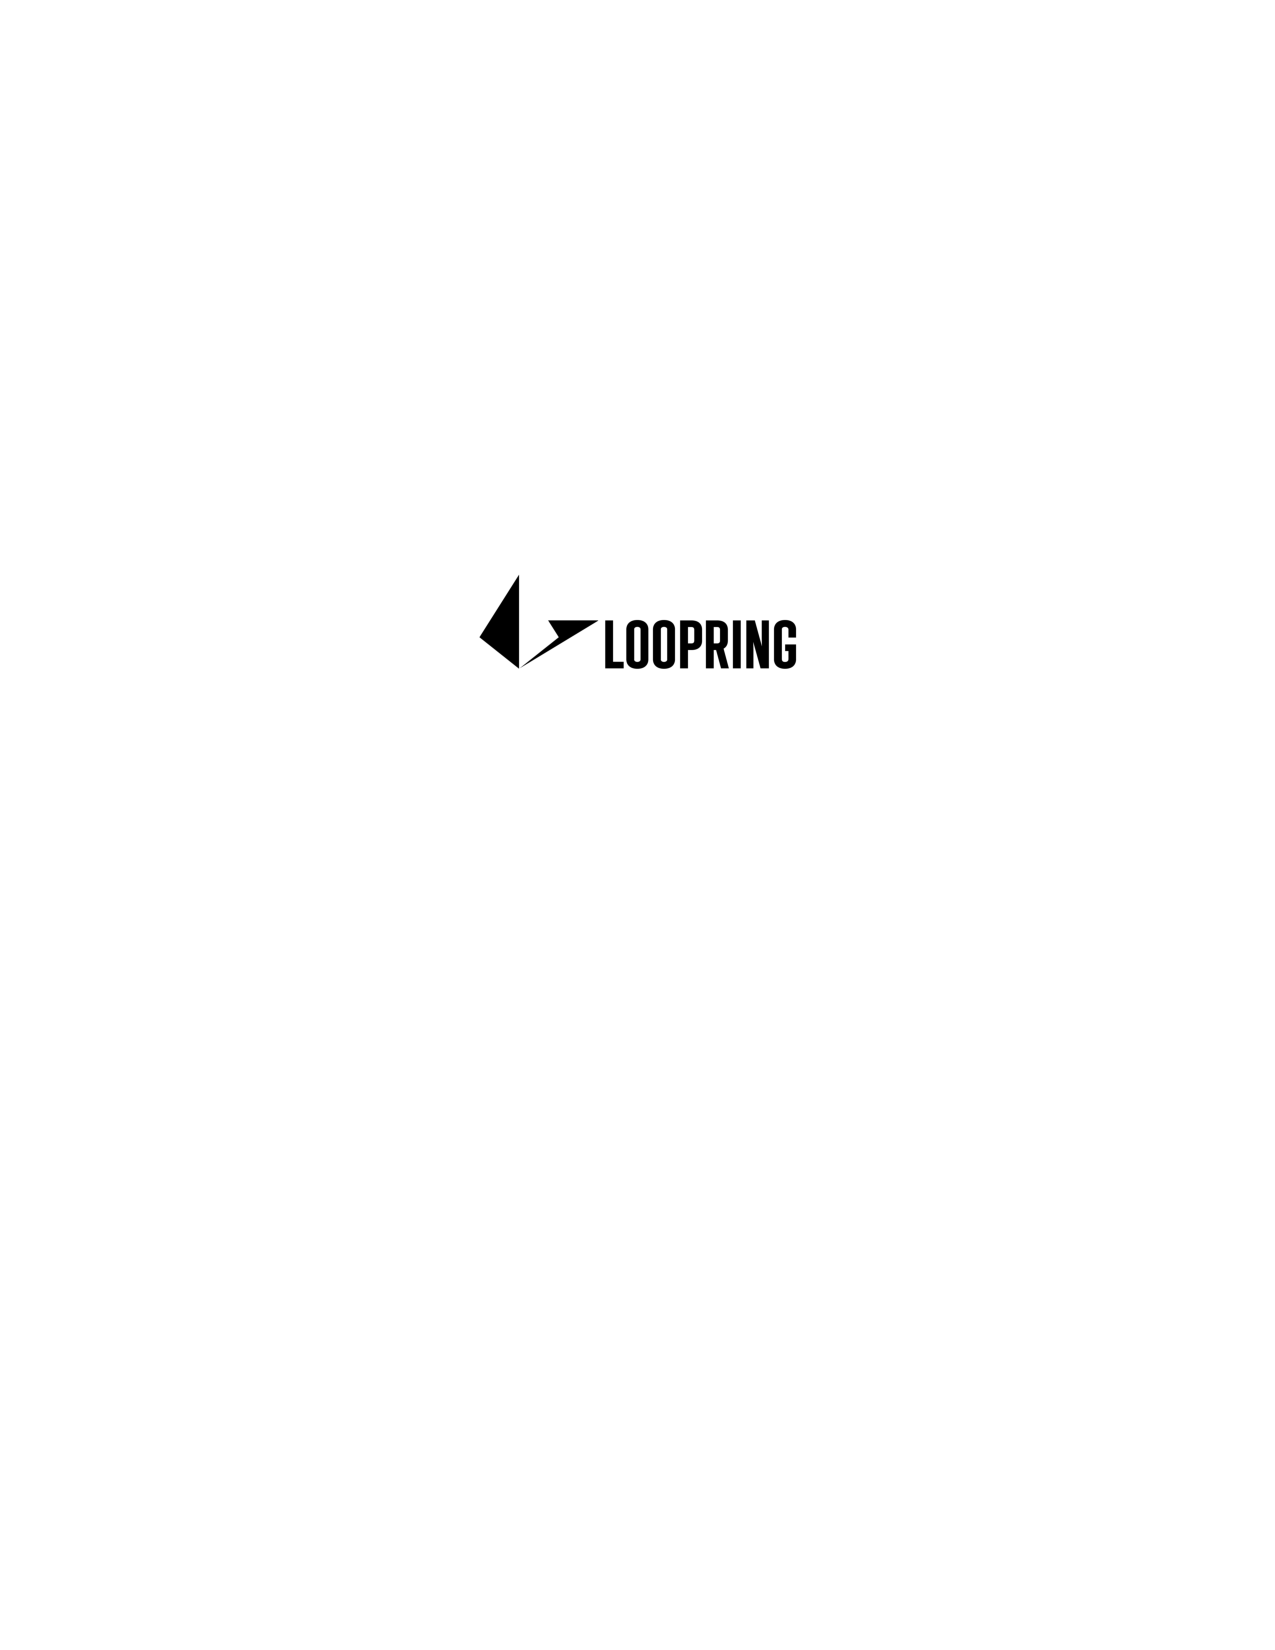
\includepdf[pages=1]{cover}


\title{\textbf{LOOPRING(루프링):\\ 탈중앙화 가상화폐 거래 프로토콜}}

\author{	
	Daniel Wang\\	
	\texttt{daniel@loopring.org}\\	
	\and	
	Jay Zhou\\	
	\texttt{jay@loopring.org}\\	
	\and	
	Alex Wang\\	
	\texttt{alex@loopring.org}\\	
	\and	
	Matthew Finestone\\	
	\texttt{matt.finestone@gmail.com}\\	
	\\	
	\texttt{https://loopring.org}	
}


\makeatletter
\def\kotex@section@format{\Large\bfseries}
\makeatother

\makeatletter
\newenvironment{tablehere}

{\def\@captype{table}}

{}

\newenvironment{figurehere}
{\def\@captype{figure}}

{}

\makeatother

\begin{document}
\maketitle
\begin{abstract}
	
	 루프팅은 탕중앙화 거래 를 구축하는 오픈 소스 프로토콜로, 거래 및 통합 작업을 수행하기 위해 공개적으로 공개되어 있는 지능형 계약뿐만 아니라 체인 아래의 참가자들이 주문을 밀접히 맺고 브로드캐스팅하는 데도 사용되고 있습니다. dApps(divisionalized computing apping)의 표준 구성 요소로 간주될 수 있는 무료이며 확장 가능한 워터마크 계약입니다. 상호 운용성 기준은 신뢰할 수 없는 익명 거래를 가능하게 합니다. 기존의 중앙 집중식 거래 계약과 비교했을 때,한 가지 중요한 개선 사항은 서로 다른 주문을 대량으로 묶고 매칭함으로써 두 개의 토큰 거래 쌍의 제약을 없애고 유동성을 높일 수 있다는 점입니다. 뿐만 아니라 초기 거래 방지를 위한 고유한 솔루션(원래 솔루션 공급업체보다 빠르게 트랜잭션을 제출하려는 불공평한 계획)이 구축되어 있습니다. 또한 블록 체인은 알 수 없으며 스마트 계약이 가능한 모든 블록 체인에 배포할 수 있습니다. 이 문서 작성 시에는 루프팅 프로토콜은 이미 Ethereum(이더리움) \cite{buterin2017ethereum} \cite{wood2014ethereum} 및 Qtum(양자 체인) \cite{dai2017smart}에서 실행되었고 NEO \cite{atterlonn2018distributed}에서 배포되었습니다.
	
\end{abstract}
\begin{multicols}{2}
\linespread{1.5}
\section{소개\label{sec:introduction}}
	\indent 블록체인 자산이 급증하면서 거래대금이 줄었던 거래 쌍방간에 이 자산을 교환하는 수요가 늘고 있습니다. 수천개의 새로운 기호화폐들이 등장-전통자산의 화폐화 포함-여기에 대한 수요가 또 커졌습니다. 투기 거래 동기에서 나오는것을 막론하고 교환을 통해 원생 응용 기호화폐 실현을 네트워크에 접근하려는 목적입니다. 디지털 통화 자산을 암호화하는 상호 교환을 실현하는 것은 보다 거대한 생태계를 위한 필수 요건입니다.실제로는 말이 통하지 않습니다. 왜냐하면 이것은 탈중앙화 프로젝트가 가지고 있는 어떤 잠재적 에너지를 위반하는 것이기 때문입니다. \cite{desotocapital} 이러한 능력을 잠금 해제(잠금 해제)하려면 소유 자산(블록 사슬이 영구적으로 유지됨)을 소유해야 할 뿐만 아니라 상호 거래 당사자가 이러한 자산을 자유롭게 이관하고 변환할 수 있어야 합니다. 따라서 신뢰할 수 없는 토큰(가치) 거래는 블록 체인 기술의 놀라운 활용 사례가 되었습니다. 그러나 오늘날까지 대부분의 암호화 디지털 통화는 기존의 중앙 집중식 거래에서 토큰 거래에 만족하고 있습니다. 따라서 비트코인 \cite{nakamoto2008bitcoin}이 강조했듯이, P2P(Point-to-Point) 전자 현금의 경우 “쌍화(P2P) 발생을 막기 위해 여전히 신뢰할 수 있는 제 3자가 필요하다면 포인트 투 포인트 현금을 사용할 수 없게 됩니다.” 마찬가지로, 신뢰할 수 있는 폐쇄적이고 중심적인 거래소에서 자산을 중앙 집중화해야 한다면 자산을 중앙 집중화할 수 없습니다. 철학적으로 중심화 교역소에서 중심화 토큰을 거래하는 것도 이념이다. 또한 Centralized Cross-Crossing 을 사용할 경우 발생할 수 있는 위험과 제한 사항도 아래에 설명되어 있습니다. DEXs(Centralized Through Deal) \cite{schuh2015bitshares} \cite{bancor} \cite{kyber}도 이러한 문제를 해결하기 위해 노력해 왔으며,블록 체인 기술을 도입하여 이러한 문제를 중대화하는 경우가 많았습니다. 몇 가지 보안상의 위험.그러나 DEX의 성능이 새로운 경제 시대의 중요한 인프라가 됨에 따라 현재 DEX는 상당한 성능 향상을 보이고 있습니다. dApp 알 수 없는 오픈 소스 프로토콜을 사용하여 이러한 인프라 구축에 모듈식 도구를 제공하는 것이 목적입니다. 
	
\section{현재 거래소 현황\label{sec:current_exchange_landscape}}

\subsection{중앙 집중화 거래소의 부족}

\indent 중앙 집중화 거래의 세 가지 주요 위험은 1) 안전성 부족 ,2) 투명성 부족,3) 유동성 부족입니다.

\indent \textbf{보안의 부재}는 종종 사용자의 개인 키(자금)로 인해 발생합니다. 중앙 집중식으로 관리할 수 있습니다. 이러한 접근 방식 때문에 사용자는 중앙 집중식 거래에서 악의적인 해커의 공격 가능성을 배제할 수 없게 되었습니다. 그러나 모든 중심 거래소가 보안 및 해커에 의해 공격될 위험이 있다는 것은 잘 알고 있지만\cite{coincheckhack}  \cite{mcmillan2014inside} 이는 대개 토큰 거래의 '입장 칩'으로 인식되고 있습니다. 중앙 집중식 거래소는 여전히 서버에 사용자 자금이 수백만 달러 이상 보관되므로 해커가 공격하는 '허니 탱크'로 남게 됩니다. 또한 거래소 개발자는 사용자 자금 관리 기관에서얼굴은 또한 정직하고 우연한 실수를 범할 수 있다. 간단히 말해 사용자는 중앙 집중식 거래소에 토큰을 부풀려도 더 이상 그의 통제를 받지 않게 됩니다 .

\indent \textbf{투명성 부족}으로 인해 사용자가 불공평하게 거래소의 부적절한 행동에 직면하게 됨우리가 주로 거래소의 운영자에 대해 악의를 품고 있다는 것입니다. 행동하는 것입니다. 실제로 사용자는 자신의 자산이 아닌 IOU 를 중앙 집중식으로 거래할 수 있습니다. 토큰이 거래소에 전달되면 거래소에 보관이 시작되고 사용자에게 IOU 계상이 제공됩니다. 따라서 사용자 이후의 모든 거래는 실제로 이러한 IOU 간의 거래입니다. 인출 시 사용자는 거래소에 자신의 IOU를 배상해 달라고 요청하며, 그 대신 트랜잭션소에서 해당 토큰을 사용자에게 전달하여 거래가 이루어지는 지갑 주소로 보냅니다. 전체 과정이 투명하지 않고, 모든 거래가 갑자기 중단될 수도 있고, 당신의 계좌를 동결하거나, 파산할 수도 있습니다. 또한 거래소에서는 제 3자에게 대여하는 것과 같이 사용자를 위해 보관된 자산을 다른 용도로 옮길 수도 있습니다. 투명성이 결여되어도사용자가 전체 자금을 손실하지만 거래 수수료가 높을 수 있음, 주문이 가장 많은 시간 동안 지연될 수 있음, 위험 관리, 주문을 앞당기는 위험 등이 있습니다.

\indent \textbf{유동성의 부족}은 거래소 운영자의 관점에서 보면, 파편화의 유동성은 새로운 거래소의 출현을 막습니다. 왜냐하면 두 개의 거래소가 시장 전체를 먹여버릴 가능성이 있기 때문입니다. 첫째, 사용자가 하나의 거래소에서 모든 거래를 운영하기를 원하기 때문에 거래 쌍이 가장 많은 거래소에서 승리합니다. 둘째, 거래 쌍마다 거래 가격 차이가 있기 때문에 주문서에서 가장 두껍게 보이는 거래소가 있습니다. 이러한 상황은 초기 유동성을 확립하기 어려우므로 신입사원이 경쟁에 참여하는 것을 방해할 수 있습니다. 이로 인해 많은 사용자들이 불만이나 대규모 해커 공격에도 불구하고 높은 시장 점유율을 차지하고 있습니다.중심 거래가 차지하는 시장 점유율이 높을수록 더 큰 공격 대상이 될 가능성이 높아진다는 점에 유의해야 합니다 .

\indent 사용자 관점에서 보면 파편화의 유동성은 사용자의 검증에 큰 영향을 미칠 수 있습니다. 중앙 집중식 거래소에서는 풀, 주문표 및 지원되는 거래팀으로만 거래를 처리할 수 있기 때문입니다. 토큰 \verb|A| 로 토큰 \verb|B| 를 거래하려면 사용자는 두 토큰 거래를 모두 지원하는 거래소를 선택하거나 별도성 거래소에서 개인 정보를 제공하여 계정을 등록해야 합니다. 또한 사용자는 BTC 또는 ETH 거래팀을 기준으로 한 단계 또는 중간 단계의 거래를 수행하고 이 프로세스 내에서 매매 가격 차이를 지불해야 하는 경우가 종종 있습니다. 마지막으로 주문 수량을 조정하지 않으면 주문 테이블 깊이가 부족하여 거래를 완료할 수 없습니다. 심지어 거래소가대량의 거래가 이루어지지만 이러한 거래의 성사나 흐름이 위조된 것이 아니라고 보장할 수는 없습니다 .\cite{fakevolume}

\indent 그 결과 유동성, 생태계가 산산조각 나면서 전통적인 금융 체계와 마찬가지로 대량의 거래가 소수의 거래소에 집중되고 있습니다. 글로벌 유동성 약속은 블록 체인의 중심 거래에는 아무런 가치가 없습니다.

\subsection{탈중심화 거래소에 존재하는 부족점}
\indent 탈중심화 거래소는 중앙 집중화 거래소와는 다릅니다. 탈중심화 거래소 에서 개인 키 ( 자산 ) 가 청크망에서 이루어지는 것을 사용자가 제어할 수 있기 때문입니다. 암호화 통화는 자체적으로 신뢰할 수 없는 기술을 사용하여 위에서 언급한 여러 보안 위험을 줄이는 데 성공했습니다. 하지만, 탈중심화 거래소에는 성능과 구조적 제약 같은 문제가 여전히 존재하고 있다.

\indent 유동성은 여전히 문제입니다. 사용자는 서로 다른 유동적 풀에서 거래를 찾아야 하기 때문입니다. DEX 또는 dApp가 상호 운용 가능한 통합 표준을 구축하지 않으면 보다 광범위한 네트워크를 통해 주문을 공유/브로드캐스팅할 수 없는 경우에도 유동성 분할이 유지됩니다. 정가 표의 유동성, 즉 복원력이 얼마나 빠른지 다시 생성할 수 있으며 이는 사용자의 최적 거래 전략에 큰 영향을 미칠 수 있습니다\cite{limitorderliquidity}.이러한 표준이 부족하면 유동성이 줄어들 뿐 아니라 잠재적으로 안전하지 않을 수 있는 독점 기술 계약의 위험에 노출될 수 있습니다.

\indent 또한 거래는 체인에서 수행되므로 DEX 는 확장성, 지연 ( 캐싱 ) 및 높은 수준의 주문 수정과 같은 기본 청크 체인의 제한을 상속합니다. 따라서 블록 체인에서 주문 테이블의 확장성이 떨어지게 됩니다. 블록 체인에서 코드를 실행하면 비용(기름비)이 발생하므로 번거로운 수의 주문을 취소하는 데 많은 비용이 소요될 수 있기 때문입니다.

\indent 마지막으로 청크 체인 주문 양식이 제공되므로 모든 거래는 광부들이 다음 청크로 포장될 때까지 기다렸다가 새 주문서에 들어가면 광부들이 모든 트랜잭션을 볼 수 있게 됩니다. 이러한 지연으로 인해 사용자는 주문을 앞당기거나 최종 거래 가격/주문 실행으로 인한 불이익을 받게 될 수 있습니다.

\subsection{혼합 솔루션 방법} 

\indent 이러한 이유로 순전히 청크 체인 기술을 기반으로 하는 거래의 모든 제약은 중앙 집중식 거래소에서 경쟁력이 떨어집니다. 따라서 탈중앙화 거래소 사슬에서 신뢰할 수 있는 특성과 중앙 집중식 신뢰가 필요 없으며, 처리 속도가 빨라야 하며 주문 처리 속도도 유연하게 유지되어야 합니다. 루프팅과 0x\cite{warren20170x} 등의 프로토콜은 체인의 중재과 주문 관리를 결합하는 솔루션을 확장시킵니다. 이러한 솔루션은 개방형 인텔리전스 계약에 따라 확장되고 여러 함수가 체인을 통해 수행됩니다. 노드 유연성을 제공하여 전체 네트워크에서 중요한 역할을 수행할 수 있도록 하여 중앙 집중식 거래소의 확장성 제한을 극복합니다. 그러나 블렌드 모델에는 여전히 결함이 있습니다. \cite{costofdecent}이 문서에서는 혼합 솔루션을 설계하는 방법에 대한 루프팅에 관한. 몇 가지 의미있는 변화를 발표하였습니다.

\section{루프팅 프로토콜\label{sec:loopring_protocol}}
\indent 루프팅 자체는 DEX 가 아니라 여러 블록 체인에 DEX 를 구축할 수 있는 모듈식 프로토콜입니다. 기존 거래소의 구성 요소를 분리하여 공개적인 인텔리전스 계약과 센터화된 참여자로 교체했습니다. 프로토콜 네트워크의 역할로는 지갑, 트렁킹, 유동 공유 통합 체인, 주문서, 루프 광부, 자산 토큰화 서비스 등이 있습니다. 각 참가자를 정의하기 전에 먼저 루프팅 주문을 이해해야 합니다. 

\subsection{주문루프\label{sec:order_ring}}
\indent 단방향 주문 모드(UDOM) \cite{coinport2014udom}는 인쇄 주문을 나타냅니다. UDOM은 주문을 토큰 거래 요청으로 봅니다. amountS/amountB(판매/구매수량) 매출이나 결제가 아닌각 주문에 대한 환율은 두 개의 토큰에 국한되므로 강력한 기능은 주문 루프에서 서로 다른 주문을 혼합하여 일치시킬 수 있다는 점입니다. 단일 거래 쌍이 아니라 최대 16개의 서로 다른 주문 유형을 통해 루프팅 계약은 유동성과 가격 성장 가능성을 크게 높여줍니다.

\begin{center}
	\begin{figurehere}
		\centering
		\tikzstyle{block} = [draw, fill=blue!20, rectangle, 
		minimum height=3em, minimum width=6em]
		\tikzstyle{sum} = [draw, fill=blue!20, circle, node distance=1cm]
		\tikzstyle{input} = [coordinate]
		\tikzstyle{output} = [coordinate]
		\tikzstyle{pinstyle} = [pin edge={to-,thin,black}]
		
		\begin{tikzpicture}[
		auto, 
		node distance=2cm,
		>=latex',
		font=\bfseries\footnotesize\sffamily,
		order/.style={
			scale=0.7,
			rectangle,
			rounded corners,
			draw=black, 
			text centered,
			%		text width=5cm,
			minimum height=12mm,
			fill=white
		},
		label/.style={
			scale=0.7
		}
		]
		% We start by placing the blocks
		
		\node [order] (order2) 
		{%
			\begin{tabular}{l}
			\textbf{주문\#2}\\
			\textbf{소유자: Y}\\
			\textbf{매출량: 9B}\\
			\textbf{매입량: 12C}
			\end{tabular}
		};
		
		\node [order, below of=order2, xshift=-3.5cm] (order1) 
		{%
			\begin{tabular}{l}
			\textbf{주문\#1}\\
			\textbf{소유자: X}\\
			\textbf{매출량: 10000A}\\
			\textbf{매입량: 2B}
			\end{tabular}
		};
		
		
		\node [order, below of=order2, xshift=3.5cm] (order3) 
	{%
			\begin{tabular}{l}
			\textbf{주문\#3}\\
			\textbf{소유자: Z}\\
			\textbf{매출량: 100C}\\
			\textbf{매입량: 160A}
			\end{tabular}
		};
		
		\draw [draw,->] (order1) -- node [label] {\textbf{7898A}} (order3);
		\draw [draw,->] (order2) -| node [label, xshift=-1.8cm] {\textbf{8B}} (order1);
		\draw [draw,->] (order3) |- node [label, xshift=1cm, yshift=0.24cm] {\textbf{98C}} (order2);
		
		\end{tikzpicture}
		
\captionof{figure}{3개 주문서를 포함하는 루프 주문}
		\label{fig:ring}
	\end{figurehere}

\end{center}

\indent 위 그림에서는 3개의 주문으로 구성된 주문 루프를 보여 줍니다. 각각의 주문서 매출을 위한 토큰(\verb|tokenS|)은 다른 주문서가 구입하고자 하는 토큰(\verb|tokenB|)입니다. 그 결과 생성되는 루프를 통해 주문하기 전에 서로의 토큰을 서로 교환할 수 있습니다. 즉, 서로의 주문이 거래로 이루어지는 것을 막을 수 있습니다. 물론 기존의 주문은 거래에 대해서는 가능하지만 본질적으로 주문 루프에서는 예외입니다.

\begin{definition}[주문 루프] $n$개의 서로 다른 토큰 $C_{0}$, $C_{1}$, $\cdots$, $C_{n-1}$ 과 $n$개 주문 $O_{0\rightarrow 1}$, $\cdots$, $O_{i\rightarrow i\oplus 1}$, $\cdots$, $O_{n-1 \rightarrow 0}$,이렇게 하면 $n$ 세대 통화의 거래 루프를 구성할 수 있습니다:$$O_{0\rightarrow 1} \rightarrow \cdots \rightarrow O_{i\rightarrow i\oplus 1} \rightarrow \cdots \rightarrow O_{n-1\rightarrow 0}\text{, }$$
	여기서 $n$ 은 루프 길이이고, $i\oplus 1 \equiv i+1 \mod n$.
\end{definition}

\indent 주문 루프는 암시적으로 지정된 초기 환율보다 높거나 같은 구성요소로 이루어진 모든 트랜잭션을 실행할 때 유효합니다. 주문 루프의 유효성을 검증하려면루트 루프팅 프로토콜 광부로부터 주문 루프를 받아야 합니다. 여기서 모든 주문의 원래 환율 곱은 1 이상이어야 합니다.

\indent Alice 와 Bob 은 자사의 토큰  \verb|A| 와 \verb|B| 를 거래하고 싶어한다고 가정해 보겠습니다. Alice에는 15개의 토큰  \verb|A|가 있고, 토큰 \verb|B| 4개 구입하려고 합니다. Bob은 10개의 토큰  \verb|B|를 가지고 있고 그것으로 \verb|B| 10개 구입하려고 합니다.

\indent 그럼, 누가 사고 누가 팔고 있는 거야? 이는 가격 정보 제공을 위한 EMC 자산에 따라 달라집니다. 토큰\verb|A|가 가격표라면 Alice는 15=3.75\verb|A|로 토큰\verb|B|를 구입하고, Bob은 30=300\verb|A|로 10개 토큰\verb|B|를 판매하는 것이다. 토큰\verb|B|가 가격표라면 Alice는 1=026667\verb|B|로 15개 토큰\verb|A|를 판매하고 있고 Bob은 10=0.333333B로 10개 토큰\verb|A|를 구입하고 있다. 따라서 구매자나 판매자는 임의로 할 수 있습니다. 첫 번째 경우 Blice는 Bob의 토큰(3.00\verb|A|)보다 3.75\verb|A| 높은 가격(3.75\verb|A|)을 지불하고, 두 번째 경우에는 Alice(0.26667\verb|B|)보다 더 높은 금액(0.3333)을 지불합니다. 구매자가 판매자의 가격보다 높거나 같은 금액을 지불하려고 하면 거래가 가능해진다는 것은 분명합니다.

\begin{equation}
{{15\over 4} \over {30\over 10}} = {{10\over 30} \over {4\over 15}}={15 \over 4} \cdot {10 \over 30} = 1.25 > 1
\end{equation}

\indent 따라서 $n$ 개의 주문으로 구성된 주문 수집을 전체 또는 부분 거래를 완료할 수 있습니다. 각 주문에 대한 지불/환율 환율 곱이 1보다 크거나 같은지 여부를 알고 있어야 합니다. 모든 $n$ 개의 주문은 일부 또는 전체로 \cite{supersymmetry} 할 수 있습니다.

\indent Alice 를 충족하기 위해 제3자 Charlie 를 도입하여 Alice가 \textit{y}$_1$개 토큰 \verb|B|을 구입하려고 \textit{x}$_1$개 토큰 \verb|A|를 두입하는 경우 Bob 은 \textit{y}$_2$개 토큰 \verb|B|를 구입하기 위해 \textit{x}$_2$개 토큰\verb|B|을 두입하는경우, Charlie는 \textit{y}$_3$개 토큰 \verb|A| 를 구입하고 \textit{x}$_3$ 개의 토큰\verb|C|을 두입해야 합니다. 모든 필수 토큰이 이미 제공되므로 다음 조건을 만족할 경우 거래가 가능합니다:

\begin{equation}
	{{x_1 \cdot x_2 \cdot x_3 \over y_1 \cdot y_2 \cdot y_3}\geq 1}
\end{equation}

\indent 루프팅 프로토콜에 대한 자세한 내용은 섹션 \ref{anatomy}을 참조하십시오.  




\section{생태계 참여자\label{sec:ecosystem}}
\indent 다음 생태계 참여자들은 중앙 집중식 거래에 필요한 모든 기능을 제공합니다.

\begin{itemize}
	
	\item \textbf{지갑}: 토큰뿐만 아니라 루프팅 네트워크로도 주문을 전송할 수 있는 일반적인 지갑 서비스 또는 연결 방식입니다. 지갑은 순차 광부와 수수료를 공유하도록 동기를 부여함으로써 계속해서 새로운 주문을 생성할 수 있습니다(\ref{sec:token}부 참조). 향후 거래는 개인 사용자 지갑 내에서 안전하게 이루어지며, 이러한 유동성 자금 풀은 EMC의 합의를 통해 연결되는 것이 중요합니다.

	\item \textbf{유동 공유 제휴 체인/트렁킹 네트워크}: 주문 및 유동성 공유를 위한 트렁킹 네트워크입니다. 연결 지점에서 Track Trunking 소프트웨어를 실행하면 기존 네트워크에 연결하여 통합 체인을 통해 다른 릴레이와 유동성을 공유할 수 있습니다. 거의 실시간 공유 주문(1-2초 청크 시간)을 실현하기 위해 EMC는 역사상 최초의 제휴 체인을 구축하고 있습니다.그리고 기존 거래의 역사를 세밀하게 조정하여 새로 만들 수 있습니다. 노드는 주문을 더 빨리 다운로드합니다. 주목할 만하게도, 릴레이는 더 이상 추가할 필요가 없습니다. 이 연합에 가입하면 유동성을 공유하지 않고 개별적으로 행동할 수 있으며 자체의 유동 공유 네트워크를 만들고 관리할 수 있습니다.

	\item \textbf{중계/거래 중제}: 중계은 지갑 또는 중계 네트워크에서 주문서를 수신하고, 공용 주문서 및 트랜잭션 내역을 유지하며, 원하는 경우 다른 트렁크(미디어 체인을 통해) 또는 중계를 선택적으로 수행네트워크 노드 브로드캐스트 주문의 노드입니다. 트렁킹의 특징은 계산이 많고 완전히 체인 아래서 실행되는 요구 사항이 아니라 트렁크의 특성입니다. \enquote{Ring-Miners}라고 하는 트렁킹은 거래의 주요 특징을 가진 트레일러로, 서로 다른 주문을 함께 연결하여 주문 루프를 생성합니다. 중계는 (1) 다른 릴레이와 의사 소통하는 방법, (2) 주문 양식을 작성하는 방법, (3) 주문 루프를 만드는 방법(광산 알고리즘) 등을 선택할 수 있는 자유입니다.

	\item \textbf{루프팅 프로토콜 스마트 계약(LPSC)}: 은 광부로부터 접수된 주문 루프를 검증하는 데 사용되는 공개적이고 무료입니다. 사용자를 대신하여 토큰을 신뢰하지 않고 결제 및 이체하고, 수수료로 광부와 지갑을 자극하고, 사건을 발표합니다. Trunking/Order 네비게이터는 이러한 이벤트를 수신하여 해당 주문 및 트랜잭션 내역을 최신 상태로 유지합니다. 자세한 내용은 부록 \ref{app:protocol_ethereum}를 참조하십시오.

	\item \textbf{자산 토큰화 서비스(ATS)}: 직접 거래가 불가능한 자산은 신뢰할 수 있는 기업 또는 조직이 관리하는 중앙 집중식 서비스입니다. 사용자가 자산(현물, 법적 통화 또는 기타 체인의 토큰)을 충전한 후 발행된 토큰을 나중에 상환할 수 있습니다. 인쇄가 적절한 솔루션이 있을 때까지 체인 간 거래 계약은 아니지만, ATS로 인해 ERC20 토큰\cite{ERC20}과 물리적 자산 및 기타 블록 체인 자산 간의 거래가 가능해졌습니다.

\end{itemize}


\section{거래 프로세스\label{sec:process}}


\begin{enumerate} 
	
	
	\item \textbf{계약 승인}: 그림 \ref{fig:process}에서 토큰\verb|B|(\verb|amountS|)를 사용자가 판매할 토큰 계약(LPSC)에 승인하기 위해 토큰을 필요로 하는 사용자 \verb|Y|가 먼저 LPSC(루프팅 프로토콜 스마트 계약)를 승인합니다. 이 작업은 사용자의 토큰을 동결하지 않습니다. 즉, 주문 실행 중에사용자들은 여전히 자신의 토큰을 자유롭게 이전할 수 있습니다.
	
	\item \textbf{주문 생성}: 주문 테이블 네비게이터의 트렁크 또는 기타 브로커와 유사한 토큰 \verb|B|와  \verb|C| 간의 환율 및 주문 테이블을 제공합니다. 사용자\verb|Y|는 완전한 지갑 인터페이스를 사용하여 매출량\verb|amountS|, 매입량 \verb|amountB| 및 기타 매개변수를 정의하여 주문(가격 제한)을 발행할 수 있습니다. 루프 광부에 대한 일정 수의 LRx 가 추가되고 LRx 의 비용이 높을수록 더 빠른 속도로 루프 광부에 의해 처리될 수 있습니다. 사용자 \verb|Y|는 자신의 개인 키로 주문의 해시 값을 서명합니다.
	
    \item \textbf{주문 브로드캐스팅}: 지갑이 주문과 디지털 서명을 하나 이상의 릴레이로 보냅니다. 그러면 중계자가 공개 주문 양식을 업데이트합니다. 계약 자체는 선착순 서비스와 같은 주문 양식의 아키텍처 원칙에 따라 필요하지 않습니다. 따라서 주문 양식을 작성할 때 네트워크에서 자유로운 설계를 수행할 수 있습니다.
    
    \item \textbf{유동 공유}: 트렁킹은 모든 통신 매체를 통해 주문을 처리할 수 있습니다.브로드캐스팅을 통해 노드 간 커뮤니케이션의 유연성을 다시 한 번 알 수 있습니다. 안정적이고 안정적인 네트워크 접속을 위해 유동 공유 릴레이 네트워크가 연합 체인에 구축되었습니다. 앞서 언급한 바와 같이 이 릴레이 네트워크는 거래 속도를 높이고 주문 참여를 최적화할 수 있습니다.

\begin{center}
	\begin{figurehere}
		\centering
		\tikzstyle{block} = [draw, fill=blue!20, rectangle, 
		minimum height=3em, minimum width=6em]
		\tikzstyle{sum} = [draw, fill=blue!20, circle, node distance=1cm]
		\tikzstyle{input} = [coordinate]
		\tikzstyle{output} = [coordinate]
		\tikzstyle{pinstyle} = [pin edge={to-,thin,black}]
		
		\begin{tikzpicture}[
		auto, 
		scale=0.7,
		node distance=2cm,
		>=latex',
		font=\bfseries\footnotesize\sffamily,
		order/.style={
			rectangle,
			scale=0.7,
			rounded corners,
			draw=black, 
			text centered,
			%		text width=5cm,
			minimum height=12mm,
			minimum width=30mm,
			fill=white
		},
		role/.style={
			circle,
			scale=0.7,
			draw=black, 
			text centered,
			%		text width=5cm,
			minimum height=12mm,
			minimum width=12mm,
			fill=white
		},
		steps/.style={
			circle,
			scale=0.7,
			draw=black, 
			text centered,
			%		text width=5cm,
			%		minimum height=12mm,
			%		minimum width=12mm,
			fill=black,
			text=white
		},
		account/.style={
			circle,
			scale=0.7,
			draw=black, 
			text centered,
			%		text width=5cm,
			minimum height=16mm,
			minimum width=16mm,
			fill=white
		},
		label/.style={
			scale=0.7
		}
		]
		
		
		\node [role] (user1)  {사용자 X};
		\node [role, below of=user1] (user2)  {사용자 Y};
		\node [role, below of=user2] (user3)  {사용자 Z};
		\node [role, below of=user3, fill=gray!20] (relay1)  {릴레이 M};
		\node [role, below of=relay1, fill=gray!20] (relay2)  {릴레이 N};
		
		
		\node [order, left of=user1, xshift=-1cm] (order1) 
		{%
			\begin{tabular}{l}
			\textbf{주문 1}\\
			\textbf{소유자: X}\\
			\textbf{매출량: 10000 A}\\
			\textbf{매입량: 2 B}
			\end{tabular}
		};
		
		\draw [draw, ->]  (user1) -- (order1) [label]{};
		\draw [bend right,->] (order1) to node [auto, scale=0.7] {} (relay1);
		\draw [bend right,->] (order1) to node [auto, scale=0.7] {} (relay2);
		% \draw [draw, ->]  (order1) |- (relay1) [label]{};
		% \draw [draw, ->]  (order1) |- (relay2) [label]{};
		
		\node [order,left of=user2, xshift=-1.5cm] (order2) 
		{%
			\begin{tabular}{l}
			\textbf{주문 2}\\
			\textbf{소유자: Y}\\
			\textbf{매출량: 9  B}\\
			\textbf{매입량: 12 C}
			\end{tabular}
		};
		\draw [draw, ->]  (user2) -- (order2) [label]{};
		\draw [bend right,->] (order2) to node [auto, scale=0.7] {} (relay1);
		\draw [bend right,->] (order2) to node [auto, scale=0.7] {} (relay2);
		% \draw [draw, ->]  (order2) |- (relay1) [label]{};
		% \draw [draw, ->]  (order2) |- (relay2) [label]{};
		% 
		\node [order, left of=user3, xshift=-2cm] (order3) 
		{%
			\begin{tabular}{l}
			\textbf{주문 3}\\
			\textbf{소유자: Z}\\
			\textbf{매출량: 100 C}\\
			\textbf{매입량: 160 A}
			\end{tabular}
		};
		\draw [draw, ->]  (user3) -- (order3) [label]{};
		\draw [bend right,->] (order3) to node [auto, scale=0.7] {} (relay1);
		\draw [bend right,->] (order3) to node [auto, scale=0.7] {} (relay2);
		% \draw [draw, ->]  (order3) |- (relay1) [label]{};
		% \draw [draw, ->]  (order3) |- (relay2) [label]{};
		
		% // The Ring
		\node [order, 
		yshift=-1.5cm,
		xshift=-2.75cm,
		below of=relay2,
		fill=gray!10,
		minimum width=4.2cm,
		minimum height=5cm] (ring) {};
		
		
		\node [order, dashed, below of=relay2,yshift=-0.2cm,xshift=-2.5cm] (order11) 
		{%
			\begin{tabular}{l}
			\textbf{주문 1}\\
			\textbf{소유자: X}\\
			\textbf{매출량: 10000 A}\\
			\textbf{매입량: 2 B}
			\end{tabular}
		};
		\node [order, dashed,below of=order11,xshift=-0.25cm,yshift=0.7cm] (order21) 
		{%
			\begin{tabular}{l}
			\textbf{주문 2}\\
			\textbf{소유자: Y}\\
			\textbf{매출량: 9  B}\\
			\textbf{매입량: 12 C}
			\end{tabular}
		};
		\node [order, dashed,below of=order21,xshift=-0.25cm,yshift=0.7cm] (order31) 
		{%
			\begin{tabular}{l}
			\textbf{주문 3}\\
			\textbf{소유자: Z}\\
			\textbf{매출량: 100 C}\\
			\textbf{매입량: 160 A}
			\end{tabular}
		};
		
		% // The blockchain
		\node [
		rectangle,
		fill=gray!20, 
		right of=user1,
		yshift=-4.5cm,
		xshift=0.1cm,
		scale=0.7,
		minimum width=3.2cm,
		minimum height=15.6cm] (blockchain) {\parbox[b][15cm]{1.3cm}{블록체인}};
		% blockchain accounts
		\node [account, right of=user1, xshift=1cm] (account1)  {계정X};
		\node [account, right of=user2, xshift=1cm] (account2)  {계정Y};
		\node [account, right of=user3, xshift=1cm] (account3)  {계정Z};
		\node [account, right of=relay1, xshift=1cm] (account4)  {계정M};
		\node [account, right of=relay2, xshift=1cm] (account5)  {계정N};
		\node [account, double, below of=account5, yshift=-1.5cm] (psc)  {LPSC};
		
		\draw [draw, ->]  (user1) -- (account1) [label]{};
		\draw [draw, ->]  (user2) -- (account2) [label]{};
		\draw [draw, ->]  (user3) -- (account3) [label]{};
		% \draw [draw, ->]  (relay1) -- (account4) [label]{};
		% \draw [draw, ->]  (relay2) -- (account5) [label]{};
		\draw [draw, double, thick]  (relay1) to node [auto, scale=0.7] {유동성 공유}  (relay2) [label]{};
		% \draw [draw, ->]  (relay1) -- (ring) [label]{};
		\draw [draw, ->]  (relay2) to node [auto, scale=0.7, xshift=-1.8cm, yshift=0.3cm] {중개거래}  (ring) [label]{};
		\draw [draw, ->]  (ring) to node [auto, scale=0.7] {커밋루프} (psc) [label]{};
		
		\draw [bend left,->] (account1) to node [auto, scale=0.7] {\textbf{7898 A}} (account3);
		\draw [bend left,->] (account2) to node [auto, scale=0.7] {\textbf{8 B}} (account1);
		\draw [bend left,->] (account3) to node [auto, scale=0.7] {\textbf{98 C}} (account2);
		
		\draw [bend left,->, dashed] (account1) to node [auto, scale=0.7] {} (account5);
		\draw [bend left,->, dashed] (account2) to node [auto, scale=0.7] {} (account5);
		\draw [bend left,->, dashed] (account3) to node [auto, scale=0.7, xshift=.5cm] {\textbf{Fee}} (account5);
		
		
		% \draw [draw,->] (order1) -- node [label] {\textbf{7898 A}} (order3);
		% \draw [draw,->] (order2) -| node [label, xshift=-1.8cm] {\textbf{8 B}} (order1);
		% \draw [draw,->] (order3) |- node [label, xshift=1cm, yshift=0.24cm] {\textbf{98 C}} (order2);
		
		\node [steps, right of=user2, xshift=-0.6cm] () {1};
		\node [steps, left of=user2, xshift=0.8cm] () {2};
		\node [steps, left of=relay2, xshift=0.3cm, yshift=1cm] () {3};
		\node [steps, left of=relay1, xshift=3.3cm, yshift=-1.6cm] () {4};
		\node [steps, below of=relay2, xshift=-0.2cm, yshift=0.4cm] () {5};
		\node [steps, right of=account3, xshift=-0.6cm] (step5) {6};
		
		\draw [bend right, ->]  (psc) to node [auto, scale=0.7, xshift=0.5cm] {settlement} (step5) [label]{};
		
		\end{tikzpicture}
		
		\captionof{figure}{루프팅 프로토콜 거래 절차}
		\label{fig:process}
	\end{figurehere}
\end{center}


\item \textbf{루프 채굴(주문 중재)}: 루프 재굴들은 다수의 추가 주문을 주어 사용자 \verb|Y|가 정하거나 더 나은 환율로 주문을 성사시키기 위해 최선을 다합니다. 루프 중재는 모든 거래가 유동성을 발휘할 수 있는 가장 큰 이유입니다. 주문에 대해 실제로 실행되는 환율이 사용자 Y에서 지정한 환율보다 높을 경우 이익 부분은 루프의 모든 주문에 의해 공유됩니다. 그리고 광부들은 수익의 일부를 추출(이익 분할 및 사용자에게 LRx 비용 반환)하거나 단순히 LRx 요금을 부과할 수 있습니다.


\item \textbf{6.검증 및 결산:}LPSC는 루프 주문을 받은 후 광부의 데이터를 검증하기 위해 여러 차례 검사를 수행합니다. 주문 루프의 전체 또는 부분적(루프에서 주문한 거래율 및 사용자 지갑의 토큰 잔액에 따라 다름)을 결정합니다. 모든 검사가 성공적일 경우 LPSC는 사용자에게 토큰을 자동으로 전달하고 그에 따라 광부와 지갑 비용을 지불합니다. LPSC에서 사용자  \verb|Y|의 지갑잔액이 부족하다고 판단하면 거래량이 비례적으로 감소합니다. 취소(전체가 단방향으로 처리되어 취소할 수 없는 주문)와 달리 토큰이 지갑 주소에 충분히 저장될 때까지 기다립니다. 감소된 주문은 초기 주문 수량으로 자동 증가합니다.
\end{enumerate}



\section{운영 유연성\label{sec:business_model}}
\indent 주목할 만하게도, 보도자료협정에 대한 개방적 기준은 참가자들에게 극적인 영향을 끼칩니다. 뛰어난 운영 유연성. 각 참가자는 LRx 수수료 ( 예 : 거래 성사 또는 기타 측정 기준 ) 에 따라 새로운 유형의 비즈니스 몰딩을 통해 가치를 창출하고 이 과정에서 일정 양의 LRx 수수료를 얻을 수 있습니다. 전체 생태계는 모듈식으로 설계되어 더 많은 애플리케이션 참고를 유도할 수 있도록 설계되었습니다.

\subsection{주문표\label{sec:order_book}}
\indent 릴레이 주문 양식을 설계할 때 어떤 방법으로든 주문을 표시하고 일치시킬 수 있습니다. 현재 EMC 의 첫 번째 주문 양식에 사용된 OTC 모드입니다. 한정된 주문은 가격에 따라서만 정렬할 수 있습니다. 즉, 주문의 타임스탬프 순서는 주문 테이블에 영향을 주지 않습니다. 하지만 중계은 주문 정렬 방식을 자유롭게 선택할 수 있으며 타임스탬프를 존중하면서 가격에 따라 주문을 진행하는 일반 중심 거래의 기본 엔진을 모방할 수 있습니다. 중계가 이러한 유형의 주문 양식을 선택하는 경향이 있는 경우, 지갑에 주문을 개별적으로 보낼 수 있도록 선택할 수 있습니다. 시간 순서에 따라 주문을 총체적으로 처리할 수 있는 중계입니다. 이러한 구성은 모두 루프팅 프로토콜에서 가능합니다.

\indent 탈중앙화 거래 프로토콜와는 달리 초기 토큰 잔액을 지불하기 위해 일정 수준의 자원을 보유하고 있어야 하는 경우가 종종 있습니다. 달리 루프팅 프로토콜의 중계는 고객이 직접 구매할 수 있는 주문을 찾기만 하면 됩니다. 초기 토큰 없이도 할 수 있습니다.

\subsection{유동성 공유\label{sec:liquidity_sharing}}
\indent 중계는 서로 공유되는 유동성(주문)을 자유롭게 설정할 수 있습니다. 우리의 연맹 사슬은 유동적 공유를 위한 하나의 방안입니다. 생태계의 회원은 선호도에 따라 자유롭게 정보를 교환할 수 있습니다. 연맹 사슬에 가입하는 것 외에 적당하다고 판단되는 한 구축하고 관리할 수 있는 능력네트워크의 유동성을 공유하고 관련 규칙 및 인센티브를 개발합니다. 이전에 지갑 구현 시나리오에서 본 주문서를 시간순으로 정렬한 것처럼 릴레이도 개별적으로 작업할 수 있습니다. 다른 중계 커뮤니케이션 협력을 선택하는 것이 네트워크 효율성을 추구하는 데 큰 이점이 있지만, 상이한 비즈니스 모델은 고유한 나눔 메커니즘을 설계하여 어떠한 방식으로든 수수료를 공유할 수 있습니다.


\section{합의서 상술\label{sec:protocol}}

\subsection{주문분해\label{anatomy}}

\indent 주문이란 거래의 목적을 설명하는 데이터 집합입니다. 루프팅 주문서는 다음과 같이 단일 주문 모드(UDOM)로 표현됩니다.

\begin{verbatim}
message Order {
address protocol;
address owner;
address tokenS;
address tokenB;
uint256 amountS;
uint256 amountB;
unit256 lrcFee
unit256 validSince; // Seconds since epoch
unit256 validUntil; // Seconds since epoch
uint8   marginSplitPercentage;  // [1-100]
bool    buyNoMoreThanAmountB;
uint256 walletId;
// Dual-Authoring address
address authAddr;
// v, r, s are parts of the signature
uint8   v;       
bytes32 r;
bytes32 s;
// Dual-Authoring private-key,
// not used for calculating order's hash,
// thus it is NOT signed.
string  authKey;          
uint256 nonce;
}
\end{verbatim}


\indent 주문 출처를 보호하기 위해 주문은 사용자의 개인 키에 의해 \verb|authAddr| 이외의 매개변수 해시에 의해 서명됩니다. \verb|authAddr| 매개변수는 주문이 상주하는 주문 루프에 사전 거래에 서명하는 데 사용됩니다(자세한 내용은 \ref{sec:dual_authoring}섹션 참조). 서명은 \verb|v|, \verb|r|, \verb|s| 필드로 표시되며 주문 매개변수와 함께 네트워크에 전송됩니다. 이는 주문 주기 전반에 걸쳐 변경이 불가능한 주문을 보장하기 위함입니다. 그러나 현재 주문 상태는 주문 주소 잔액과 기타 변수에 기초하여 평가됩니다.



\indent UDOM에는 가격이 포함되지 않습니다(기본적으로 부동 소수점이어야 함). 대신 \verb|rate| 또는 $r$이라는 용어를 사용하여 \verb|amountS|/\verb|amountB|로 표현합니다. 환율은 부동 소수점 숫자가 아니라 표현식이며 필요한 경우에만부호 없는 다른 정수를 사용하여 계산되어 모든 중간 결과를부호 없는 정수로 유지하여  계산 정밀도를 높입니다.

\subsubsection{매입량}

\indent 순환경로에 있는 광부들이 일단 주문을 하면, 더 나은 주문을 발견할 수 있을 것입니다. 사용자가 지정된 매입보다 더 많은 \verb|tokenB|를 얻을 수 있도록 하는 행 환율입니다. 그러나 \verb|buyNoMoreThanAmountB| 함수가 \verb|True|로 설정된 경우 계약을 통해 사용자가 \verb|amountB|를 초과하지 않는 \verb|tokenB|를 받을 수 있습니다. 따라서 UDOM의 \verb|buyNoMoreThantokenB| 함수는 주문이 완전히 거래되는 시기를 결정합니다. \verb|buyNoMoreThantokenB| 매개 변수에는 거래 의사를 보다 자세하게 표현할 수 있는 기존의 거래 주문보다 \verb|amountS| 또는 \verb|amountB|에 대한 상한이 있습니다.

\indent 예를 들어 \verb|amountS| = 10이고 \verb|amountB| = 2인 경우 환율은 $r$ = 10/2 = 5가 됩니다. 따라서 사용자는 토큰 하나와 \verb|tokenB|를 교체하기 위해 5 개의 \verb|tokenS| 를 판매할 수 있습니다. 루프 광부들이 일단 접속했을 때 사용자에게 더 나은 환율 4 가 제공되어 사용자가 2 개 대신 2.5 명을 받을 수 있게 되었습니다. 그러나 사용자가 2개의 \verb|tokenB|만 구입하고 \verb|buyNoMoreThanAmountB|가 \verb|True|로 설정된 경우 LPSC는 환율에 따라 거래를 4개, 사용자가 4개의 \verb|tokenS|를 사용하여 1개의 \verb|tokenB|를 구입하면 결과적으로 2개의 \verb|tokenS|를 절감합니다. 기억하세요, 여기서는 아직 광산작업비를 고려하고 있지 않습니다.(\ref{sec:fee_model}섹션 참조).

\indent 사실, 우리가쓰는


\begin{verbatim}
Order(amountS,tokenS,
      amountB,tokenB,
      buyNoMoreThantokenB)
\end{verbatim}

\indent 명령어는 ETH/USD 거래 시장의 기존 거래 방식에서 볼 수 있는 간단한 형태의 주문을 의미합니다. 아래의 첫 번째 및 세 번째 주문으로 표시하지만 나머지 2개는 주문으로 표현할수 없습니다:

\begin{enumerate}
	\item 300USD/ETH 가격에 10개의 ETH 판매되며 다음과 같이 표시할 수 있습니다: 
 
 \verb|Order(10, ETH, 3000, USD, False)|.
	\item 300USD/ETH 가격에 10개의 ETH를 판매하면 3000USD를 얻을 수 있습니다.다음과 같이 표시할 수 있습니다 \verb|Order(10,ETH, 3000, USD, True)|.
	\item 300USD/ETH 가격에 10개의 ETH를 구입하면 다음과 같이 표시할 수 있습니다 \verb|Order(3000, USD, 10, ETH, True)|.
	\item 300USD/ETH 가격에서 3000USD소비하고 더 많은 ETH를 구입하면 다음과 같이 표시할수 있습니다 \verb|Order(3000, USD, 10, ETH, False)|.
\end{enumerate}



\subsection{루프 검증\label{sec:ring_verification}}

\indent LPSC는 환율 또는 트랜잭션 수량 계산 작업을 수행하는 것이 아니라 루프 광부의 값을 받아들이고 검증해야 합니다. 이러한 계산은 (1) 이더넷 네트워크의 solidity\cite{dannen2017introducing}언어와 같은 지능형 계약의 프로그래밍 언어와 부동 소수점 계산을 지원하지 않는 주된 두 가지 이유로 루프 광부에서 수행됩니다. 특히 작업 로드 증명 매커니즘  $pow(x, 1/n)$ (하나의 부동 소수점 수에 대해 n제곱 루트 계산) (2) 청크 체인의 계산 및 비용을 줄이기 위해 체인 아래에서 계산을 수행하는 것이 가장 좋습니다.


\subsubsection{하루프 검사\label{sec:sub_ring_check}}
\indent 이 단계는 자금 조달자가 주문 루프를 통해 새로운 주문을 수행하여 마진을 부당하게 얻지 못하도록 하기 위한 단계입니다. 본질적으로, 루프 광부들이 합법적인 주문 루프를 하나 발견하면, 사용자의 이익 (환율 할인 ) 을 위해 다른 주문을 주문 루프에 추가하는 것이 가능해질 수 있습니다. 그림 \ref{fig:subring}과 같이 $x1$, $y1$, $x2$ 및 $y2$를 신중하게 계산하여 루프의 모든 주문에 대한 환율 곱하기가 정확히 1이면 환율 할인이 없습니다.
\begin{center}
	\begin{figurehere}
		\centering
		\tikzstyle{block} = [draw, fill=blue!20, rectangle, 
		minimum height=3em, minimum width=6em]
		\tikzstyle{sum} = [draw, fill=blue!20, circle, node distance=1cm]
		\tikzstyle{input} = [coordinate]
		\tikzstyle{output} = [coordinate]
		\tikzstyle{pinstyle} = [pin edge={to-,thin,black}]
		
		\begin{tikzpicture}[
		auto, 
		node distance=2cm,
		>=latex',
		font=\normalfont,
		order/.style={
			scale=0.8,
			rectangle,
			rounded corners,
			draw=black, 
			text centered,
			%		text width=5cm,
			minimum height=12mm,
			fill=white
		},
		label/.style={
			scale=0.7
		}
		]
		% We start by placing the blocks
		
		\node [order] (order2) 
		{%
			\begin{tabular}{l}
			\textbf{주문 2}\\
			\textbf{소유자: Y}\\
			\textbf{매출량: 9B}\\
			\textbf{매입량: 12C}
			\end{tabular}
		};
		
		\node [order, below of=order2, xshift=-3.5cm] (order1) 
		{%
			\begin{tabular}{l}
			\textbf{주문 1}\\
			\textbf{소유자: X}\\
			\textbf{매출량: 10000 A}\\
			\textbf{매입량: 2 B}
			\end{tabular}
		};
		
		
		\node [order, below of=order2, xshift=3.5cm] (order3) 
		{%
			\begin{tabular}{l}
			\textbf{주문 3}\\
			\textbf{소유자: Z}\\
			\textbf{매출량: 100 C}\\
			\textbf{매입량: 160 A}
			\end{tabular}
		};
		
		\node [order, below of=order3, yshift=-1.5cm, fill=gray!20] (order4) 
		{%
			\begin{tabular}{l}
			\textbf{주문 4}\\
			\textbf{소유자: M}\\
			\textbf{매출량: x1 A}\\
			\textbf{매입량: y1 B}
			\end{tabular}
		};
		
		
		\node [order, below of=order1, yshift=-1.5cm, fill=gray!20] (order5) 
		{%
			\begin{tabular}{l}
			\textbf{주문 5}\\
			\textbf{소유자: M}\\
			\textbf{매출량: x2 C}\\
			\textbf{매입량: y2 A}
			\end{tabular}
		};
		
		\draw [draw,->] (order1) -- node [label, xshift=2cm] {} (order5);
		\draw [draw,->] (order2) -| node [label, xshift=-1.6cm] {} (order1);
		\draw [draw,->] (order3) |- node [label, xshift=1cm] {} (order2);
		\draw [draw,->] (order4) -- node [label, xshift=2cm] {} (order3);
		\draw [draw,->] (order5) -- node [label, yshift=0.2cm] {} (order4);
		
		\end{tikzpicture}
		
		\captionof{figure}{하위 루프를 포함하는 루프 주문}
		\label{fig:subring}
	\end{figurehere}
\end{center}

\indent 이러한 방식은 네트워크 전체에서 위험은 전혀 없으나 아무런 가치도 가져오지 않으며 순환 광부의 부정 행위로 간주합니다. 이를 방지하기 위해 루프투 계약에서는 합법적인 루프 내에 하위 루프가 없어야 합니다. 이를a 보장하기 위해 LPSC는 토큰을 두 번 매입하거나 두 번 판매할 수 없도록 합니다. 위 그림에 나와 있는 것처럼 토큰 A는 두 번 판매된 토큰 A와 두 번 거래되는 것으로 허용되지 않습니다.

\subsubsection{거래 성사율 검사\label{sec:fill_rate_check}}


\indent 주문 루프에서 환율 계산 은 반드시 LPSC 가 정확한 검증을 위해 반드시 수행해야 하는 루프 광부의 필요성을 위에서 설명했습니다. 먼저 LPSC는 각 주문에서 광부의 매입률이 사용자가 설정한 매입율보다 작거나 같은지 검증하여 사용자가 거래에서 최소한 필요한 환율 이상을 요구할 수 있도록 합니다. LPSC는 먼저 각 주문에서 광부의 매입률이 사용자가 설정한 매입률보다 작거나 같은지 확인하며, 이에 따라 사용자는 거래에서 최소한의 환율을 요구할 수 있습니다. 둘째, 환율이 결정되면 LPSC는 주문 루프의 모든 주문을 동일한 환율 할인을 받는 비율입니다. 예를 들어, 환율 할인율이 $\gamma$ 인 경우\ 주문당\ 가격은\ 다음과\ 같습니다.

$r_{0\rightarrow 1} \cdot (1-\gamma)$, $r_{1\rightarrow 2} \cdot (1-\gamma)$, $r_{2 \rightarrow 0} \cdot (1-\gamma)$
그리고\ 아래조건을\ 만족해야\ 합니다:\\
\begin{equation}
r_{0\rightarrow 1} \cdot (1-\gamma)\cdot r_{1\rightarrow 2} \cdot (1-\gamma) \cdot r_{2 \rightarrow 0} \cdot (1-\gamma) = 1
\end{equation}
따라서:\\
\begin{equation}
\gamma = 1- \frac{1}{\sqrt[3]{r_{0\rightarrow 1} \cdot r_{1\rightarrow 2} \cdot r_{2\rightarrow 0}}}\text{.}
\end{equation}
\indent 따라서 만약 모든 거래중 n개 주문이 포함되여 있다면 \texttt{discount(할인)}은\\
\begin{equation}
\gamma = 1- \frac{1}{\sqrt[n]{\prod_{i=0}^{n-1} r^i}} \text{,}
\end{equation}

 $r^i$는 $i$번째 주문의 회전율을 나타냅니다. 분명히 할인율이 $\gamma \ge 0$인 경우에만 이러한 주문이 성사되고 제\textit{i}주문($O^i$)의 실제 환율은$\hat{r^i} = r^i \cdot (1-\gamma)$, $\hat{r^i}\le r^i$ 입니다.
 
\indent 앞서 살펴본 바와 같이  Aice는 15개의 토큰 \verb|A|를 가지고 있고, 또 4개의 토큰\verb|B|를 구입했고Bob은 10개의 토큰\verb|B|를 가지고 있으며 30개의 토큰 \verb|A|를 구입하고 싶습니다. 토큰 \verb|A|가 가격 책정 기준이라면, Alice는 $\frac{15}{4}$ = 3.75\verb|A|, 의 가격으로 토큰\verb|B|를 구입하는 것입니다. Bob 은$\frac{30}{10}$ = 3.00\verb|A| 가격으로 토큰 \verb|B|를 판매하고 있습니다. 할인가격은:$\frac{150}{120}$ = 1.25 즉 $\frac{1}{1.25}$ = 0.8 = $(1 −- \gamma)^2$. 따라서 실제 거래에서 서로 공평한 환율은 $\sqrt{0.8}$ $\cdot$ 3.75 $\approx$ 3.3541 토큰 \verb|A| per 토큰 \verb|B|.\\
\indent Bob 은 4개의 토큰\verb|B|가 13.4164개의 토큰 \verb|A|를 받았으며, 그가 4개의 토큰 \verb|B|로 예상한 12개 토큰\verb|A|보다 더 많은 것을 받았습니다. Alice 는 4 개의 토큰\verb|B| 를 받았지만 13.4164 개의 토큰 \verb|A| 만 기대했던 15 개의 토큰 \verb|A| 보다 낮습니다. 일부 이익은 광부에게 수수료로 보상됩니다.(\ref{sec:fee_model}항 참조). 


\subsubsection{거래 추적 및 취소}

\indent LPSC에 특정 거래의 일부 또는 전체를 전송하여 주문을 취소할 수 있습니다. 주문 세부 사항과 계획 취소 수량도 포함되어야 합니다. 그런 다음 LPSC는 취소해야 할 수량을 보존하고 네트워크에 \verb|OrderCancelled| 이벤트를 게시하는 딜을 기록합니다. LPSC는 주문 해시 값을 식별자로 사용하여 거래가 성사되고 취소된 수량을 지속적으로 추적하여 해당 값을 저장합니다. \verb|OrderCancelled| / \verb|OrderFilled| 이벤트는 데이터가 변경될 때마다 공개적으로 액세스할 수 있습니다.LPSC에서는 이러한 값을 축소된 단계에서 추적하는 것이 중요합니다.

\indent 또한 LPSC는 \verb|OrdersCancelled|를 사용하여 사용자 주소의 모든 거래 쌍 주문을 취소할 수 있는또, \verb|AllOrdersCancelled| 사용자 주소의 모든 거래 쌍 주문을 쉽게 취소할 수 있습니다. 

\subsubsection{주문 감소\label{sec:order_scaling}}
\indent 과거 거래량, 취소량 및 발신자 계정의 현재 잔액을 기준으로 주문을 공제할 수 있습니다. 전체 프로세스는 위에서 언급한 주문 특징에 따라 매입/매출량이 가장 적은 주문을 파악하여 주문 단일 루프에서 모든 거래량을 줄이는 데 참조할 수 있어야 합니다.

\indent 각 주문에 대한 거래량을 계산하는 데 도움이 되는 최소의 주문을 찾으십시오. 예를 들어, \textit{i}번째 주문이 최소 주문인 경우 각 주문에서 판매된 토큰 수량 $\hat{s}$와 각 주문에서 구매한 토큰 수량 $\hat{b}$ 는 다음과 같이 계산됩니다.

\[
\begin{split}
&\hat{s}^{i}=\overline{s}_i\text{, } \hat{b}^{i}=\hat{s}^{i}/ \hat{r}^i\text{, }\text{;}\\
&\hat{s}^{i\oplus 1}=\hat{b}^i\text{, } \hat{b}^{i\oplus 1}=\hat{s}^{i\oplus 1}/ \hat{r}^{i\oplus 1}\text{;}\\
&\hat{s}^{i\oplus 2}=\hat{b}^{i\oplus 1}\text{, } \hat{b}^{i\oplus 2}=\hat{s}^{i\oplus 2}/ \hat{r}^{i\oplus 2}\text{;}\\
& ...
\end{split}
\]

여기서 $\overline{s}_i$는 주문의 일부에 대한 계정 잔액입니다.

\indent 실제 운영에서는 루프의 임의 주문을 안심하고 가정할 수 있습니다. 최소의 주문을 한 다음 두 번 이상 주문을 루프에 순환시켜 주문별 거래량을 산출할 수 있습니다.\\
\indent 예를 들어 계약이 성사될 수 있는 최소 수량이 최초 주문의 5\%인 경우 단일 루프의 모든 거래 건수는 5\%로 감소합니다.거래가 완료되면 거래가 성사될 때까지 최소 거래량으로 간주되는 주문은 이미 완전히 거래가 성사된 상태여야 합니다.

\subsection{루프중재\label{sec:settlement}}

\indent 주문 루프가 이전 검증을 모두 통과하면 주문 루프가 종료되고 거래가 완료됩니다. 이는 모든 $n$ 개 주문이 그림 4 와 같이 마감된 하나의 주문 루프를 형성함을 의미합니다.

\begin{center}
	\begin{figurehere}
		\centering
		\begin{tikzpicture}[
		circle/.style={
			scale=0.75,
			rounded corners,
			draw=black, 
			text centered,
		}
		]
		
		\def \n {6}
		\def \m {4}
		\def \radius {1.4cm}
		\def \margin {12} 
		
		\foreach \s in {1,...,\m}
		{
			\node[draw, circle] at ({360/\n * (\s - 1)}:\radius) {$O^\s$};
			\draw[<-, >=latex] ({360/\n * (\s - 1)+\margin}:\radius) 
			arc ({360/\n * (\s - 1)+\margin}:{360/\n * (\s)-\margin}:\radius);
		}
		
		\node[draw, circle] at ({360/\n * 4}:\radius) {$O^5$};
		\draw[<-, dashed, >=latex] ({360/\n * 4+\margin}:\radius) 
		arc ({360/\n * 4+\margin}:{360/\n * (5)-\margin}:\radius);
		
		\node[draw, circle] at ({360/\n * 5}:\radius) {$O^n$};
		\draw[<-, >=latex] ({360/\n * 5+\margin}:\radius) 
		arc ({360/\n * 5+\margin}:{360/\n * (6)-\margin}:\radius);
		
		
		\end{tikzpicture}
		
	\captionof{figure}{루프 중재}
	\label{fig:settlement}
	\end{figurehere}
\end{center}

\indent 딜을 성사시키기 위해 LPSC 는\verb|TokenTransferDelegate| 지능형 계약을 호출합니다. 이러한 에이전시 메커니즘을 도입하면 서로 다른 모든 계약 버전이 아닌 에이전시만 주문할 수 있으므로 계약 인텔리전스 계약을 쉽게 업그레이드할 수 있습니다.

\indent 주문 루프의 각 주문에 대해 실행에 따라다음 또는 이전 주문에 대해 일정 금액의 \verb|tokenS|를 지불해야 합니다. 그런 다음 광부들이 선택한 요금 패턴에 따라 광부들에게 비용을 지불합니다. 마지막으로, 모든 교차가 쉽게 완료되면 \verb|RingMined| 이벤트가 게시됩니다.

\subsubsection{이벤트 게시\label{sec:events}}

\indent 루프팅 계약 이벤트 게시눈 중계, 주문 네비게이터 및 기타 딜러가 가능한 한 효율적으로 주문 업데이트를 수신할 수 있도록 하는 이벤트입니다. 게시된 이벤트는 다음과 같습니다:

\begin{itemize}
	\item \textbf{OrderCancelled}: 특정 주문이 취소되었습니다.
	\item \textbf{OrdersCancelled}: 사용자 주소 아래의 거래는 모든 주문서가 취소되었습니다.
	\item \textbf{AllOrdersCancelled}: 사용자 주소 아래의 모든 거래 등록이 취소되었습니다.
	\item \textbf{RingMined}: 주문 루프 중 하나가 성공적으로 이루어졌습니다. 이 이벤트 에는 루프의 각 토큰 이체에 대한 자세한 데이터가 포함되어 있습니다.
\end{itemize}


\section{LRx 토큰\label{sec:token}}

\indent LRx는 도로의 일관된 토큰 기호입니다. LRC는 이데리움 네트워크 의 도로 토큰이고, LRQ는 양자 체인 네트워크의 도로 토큰이며, LRN은 NEO 네트워크의 도로 토큰입니다. 도로판이 계속해서 다른 공용 체인에 배포됨에 따라 향후 다른 유형의 LRx 토큰도 도입될 예정입니다.

\subsection{유료 모드\label{sec:fee_model}}
\indent 사용자가 주문을 생성하면 광부에게 지불할 수 있는 수수료와 함께 \verb|marginSplitPercentage|의 마진 비율(\verb|marginSplitPercentage|)과 함께 일정 수의 LRx가 수수료로 지불됩니다. 이것을 "분윤비율"이라고 부릅니다. 다음 중 하나를 선택하십시오(수수료 또는 윤률분). 방식은 전적으로 광부의 자율에 의해 결정된다.

\indent 다음 그림은 분할 배율 조정 그림입니다:

\begin{center}
	\begin{figurehere}
		\centering
		\begin{tikzpicture}[
		scale=1,
		font=\bfseries\footnotesize\sffamily,
		classical/.style={thick,<->,shorten >=2pt,shorten <=2pt,>=stealth},
		oneway/.style={->,dashed,shorten >=2pt,shorten <=2pt,>=stealth}
		]
		% Draw axes
		\draw [->,thick] (0,1) node (yaxis) [above] {$$}
		|- (6.2,0) node (xaxis) [right] {$$};
		
		\draw
		(4,0) coordinate (A)
		(4,1) coordinate (A2)
		(4.8,-0.6) coordinate (B)
		(4.8,1) coordinate (B2)
		(6,-0.6) coordinate (C)
		(6,1) coordinate (C2);
		
		\fill [draw=none, fill=gray!20] 
		(4.8, 0) rectangle (6, 1);
		
		\fill [draw=none, fill=gray!10] 
		(0, -0.6) rectangle (4.8, 0);
		\draw[thick] (0, -0.6) -- (0, 0.6) node[below]{$$};
		\draw[thick, thin] (A) -- (A2) node[below]{$$};
		\draw[thick, thin] (B) -- (B2) node[below]{$$};
		\draw[thick] (C) node[below, xshift=0.5cm]{총구입량} -- (C2) ;
		
		\draw[classical] (0, 0.5) -> (4, 0.5) node[below]{$$};
		\draw[classical] (4, 0.75) -> (4.8, 0.75) node[below]{$$};
		\draw[classical] (4, 0.25) -> (6, 0.25) node[below]{$$};
		
		\draw[oneway] (2, 1.2) node[above]{초기주문량} -- (2, 0.5);
		\draw[oneway] (4.4, 2.2) node[above]{추가주문량} -- (4.4, 0.75);
		\draw[oneway] (5.4, 1.6) node[above]{분윤비율} -- (5.4, 1);
		\draw[oneway] (5, -1.2) node[below]{이익} -- (5, 0.25);
		\draw[oneway] (2.4, -1.2) node[below]{실제구입량} -- (2.4, -0.5);
		\end{tikzpicture}
		
	\captionof{figure}{60\%의 분윤율}
		\label{fig:marginsplit}
	\end{figurehere}
\end{center}

\indent 주문 루프에서 이익률이 너무 낮으면 광부들은 LRx 모드를 선택합니다. 반면에 수익이 너무 커서 LRx 비용을 훨씬 초과할 경우 광부들은 분윤율 패턴을 선택할 수도 있지만 여기서 제한되는 또 다른 제한 사항은 광부들이 분윤율 패턴을 선택하는 경우입니다. 고객은 사용자가 광부에게 지불해야 할 LRx 비용에 해당하는 사용자(주문 생성자)에게 비용을 지불해야 합니다. 이렇게 하면 광부 선택 점수 윤률 패턴의 문지방이 LRx 비용 패턴의 두 배로 높아지고 LRx 모델을 선택하는 경향이 커집니다. 이로써 광부들은 낮은 수익의 루프 주문을 고정 수익으로 전환하여 높은 수익의 루프 주문에서 적은 수의 수익을 거둘 수 있게 되었습니다. 이 경우 시장이 성장하고 성장함에 따라 수익성이 높은 루프 주문이 감소할 것으로 예상하므로 인센티브로 LRx를 고정해야 합니다.


\indent 최종적으로 다음과 같은 그래프를 얻을 수 있습니다.


\begin{center}
	\begin{figurehere}
		\centering
		\begin{tikzpicture}[
		font=\bfseries\footnotesize\sffamily,
		oneway/.style={->,dashed,shorten >=2pt,shorten <=2pt,>=stealth},
		scale=1]
		% Draw axes
		\draw [<->,thick] (0,2.7) node (yaxis) [above] {$y$}
		|- (5,0) node (xaxis) [right] {$x$};
		
		\draw
		(1,1) coordinate (A)
		(2,1) coordinate (B);
		
		
		\draw[thick] (B) -- (3.7,2.7);
		\draw[dotted] (B) -- (2,0) node[below] {$2f$};
		\draw[dotted] (A) -- (1,0) node[below] {$f$};
		\draw[thick,color=gray!70] (0,0) -- (2.7,2.7);
		\draw[thick] (0,1) node[left] {$f$}--(B) node[     ]{$$};
		\draw[oneway] (4,1) node[right]{예상 광산 수익} -- (3, 2);
		
		
\end{tikzpicture}
\captionof{figure}{루프팅 요금 모드}
\label{fig:feemodel}
\end{figurehere}
\end{center}
		
\indent 여기서 $f$는 LRx 비용, $x$는 분윤율, $y$는 광산 수익입니다. 실선은 $y=max(f, x-f)$를 나타내고, 한 주문의 LRx 비용이 $0$이면 $y=max(0, x - 0)$ 방정식으로 표시됩니다. 간단히 말해서 $y = x$를 나타내는 회색 실선입니다.


\indent 이에 따른 결과는 다음과 같습니다:
\begin{enumerate}
      \item 분수 비율이 0이면 광부들은 별로 매력이 없는 LRx 요금 패턴을 선택하고 상을 받습니다.
      \item LRx 비용이 0이면 실선이 회색으로 표시됩니다. 이제 광부 의 수익은 일반 선형 모델이 됩니다.
      \item 분할 비율 수입이 LRx 비용 패턴의 두 배 이상인 경우 광부 는 사용자에게 LRx를 지급할 분윤율 패턴을 선택합니다.
\end{enumerate}

\indent 주의해야 할것은 LRx 비용이 0이 아니면 광부들이 어떤 방식을 택하든, 광부와 주문 개시자가 LRx를 송금하기 전에 항상 LRx 이체가 발생합니다. 광부들은 LRx 요금을 받기로 결정했습니다. 또는 주문 개시자에게 LRx 요금을 반환하고 비율 조정 요금을 지불해야 합니다. 

\indent 게다가, 광부들은 또한 지갑과 일정 비율의 비용을 공유할 것입니다. 사용자지갑을 통해 주문을 시작하고 최종적으로 거래가 성사되면 요금이나 윤활 비율에 따라 지갑에 보상이 발생합니다. 이 설정은 모듈화되어 있지만, 필요에 따라 고유한 비즈니스 모델이나EMC는 광부의 약 20\%-25\%의 수익을 내는 것을 선호합니다. 지갑은 집선인협의의 주요 목표이긴 하지만 그 자체로는 수입원이 거의 또는 전혀 없기 때문입니다.

\subsection{탈중앙화자치}

\indent 기본적으로 PIP(People-in-print)는 특정 목표를 달성하기 위해 구성원 간의 협력에 의존하는 소셜 프로토콜입니다. 이와 같은 암호-경제 프로토콜은 이와 다르지 않지만, 실질적으로 동일한 조정 문제 메커니즘\cite{vitalikgovernance}과 균형 조정 및 이성적인 보호를 통해 매우 유용하게 사용될 수 있습니다. 따라서 LRx 토큰의 용도는 단순히 비용을 지불하는 것이 아니라 네트워크 참여자들의 재정적 인센티브를 조정하는 데도 사용됩니다. 이러한 조정은 모든 협정을 광범위하게 채택하는 데 필요하며, 대체 협정에서는 특히 중요합니다. 마크 협정의 최종 성공 여부는 건전한 센터화 생태계의 유동성을 높이는 데 크게 달려 있기 때문입니다.

\indent LRx 토큰은 중앙 집중식 자율화를 통한 계약 갱신에 사용됩니다. 미래에는 지능형 계약 업데이트는 토큰 소유자의 책임으로 처리되므로 일관성, 보안 및 비호환성을 보장하고 유동성 손실 위험을 줄일 수 있습니다. 지능형 계약이 배포되면 수정할 수 없게 되므로 dApp 또는 최종 사용자는 더 이상 사용되지 않는 버전과의 상호 작용이 계속되고 최신 버전을 사용할 수 없게 될 수 있습니다. 계약의 위험. 업그레이드 기능은 시장 및 기본 블록 체인의 발전에 적합해야 하므로 계약 성공의 핵심입니다.LRx 주주의 거버넌스 거버넌스 인텔리전스 기능을 통해 dApp, 최종 사용자 또는 지능형 계약 추출에 대한 과도한 의존 없이 계약 인텔리전스 계약을 업그레이드할 수 있습니다. LRx 토큰의 총 발행량은 고정되어 있습니다. LRC를 예로 들면, 일정 비율의 토큰은 도로 인쇄 재단이 소유하고, 일정 비율의 토큰은 지역사회의 성장을 지원하기 위한 자금으로 사용됩니다.

\indent 그러나 LRx 토큰 소유주만이 루프팅 계약 협정의 진행 방향을 파악한 유일한 주주가 아닙니다. 중계/루프 광부, 지갑, 개발자 및 그 참가자는 전체 생태계의 일부입니다. 루프팅 협정의 발전도 반드시 그들의 의견과 건의를 들어야 합니다. 실제로 이러한 참가자는 LRx 토큰을 가지고 자신의 역할을 수행할 필요가 없기 때문에(구매자/구매자 및 소매업자 역할은)(초기 토큰 준비금은 강제 사항이 아니므로 다른 방법을 통해 그들의 이익을 충족해야 합니다. 또한, “단순한” 토큰 기반 투표, 즉 체인에서 이루어지든 사슬에 묶여 있든 모두 불완전하며, 이는 저투표율과 토큰 전환 집중에 따른 위험을 초래할 수 있기 때문입니다. 따라서 상호 합의를 토대로 표준 의사 결정 프로세스를 수립하는 데 필요한 기업 내부 규정 모델을 구축하는 것이 EMC 의 목표입니다. 조정기구를 사용하여 참가자 집단을 수집할 수 있으며 사전 정의된 프로토콜 통신 지점의 다양한 음성도 수집할 수 있습니다. 이러한 성과가 이루어짐에 따라 루프팅재단은 필연적으로 계약 개발자에서 계약 관리자로 발전하게 될 것입니다.

\section{사기 및 공격 보호}
\subsection{사전 교역을 방지하다\label{sec:dual_authoring}}

\indent 중심화 거래에서 사전 거래란 다른 지점의 딜을 복제하여 미성결 거래 풀(mimpool)을 재결합하는 것을 의미하며, 이 경우 더 높은 거래 비용(유료)을 지정하여 실현할 수 있습니다. 사전 거래(및 기타 주문 압류 계약)의 루프팅 계약 주요 주문 절도: 선제 거래자, 거래 성사되지 않은 순환, 잇대기 거래에서 채취. 하나 이상의 주문우선적으로는 선구자가 거래가 성사되지 않은 시점에서 전체 주문 루프를 빼내야 합니다.


\indent 제출된 루프 거래(submitRing)가 확인되지 않고 여전히 거래 풀의 미성별 상태일 때이러한 거래는 쉽게 발생할 수 있으며, 광부 주소 \verb|minerAddress|를 광부 주소 \verb|minerAddress|로 대체하여 자신의 주소(the \verb|filcherAddress|)를 쉽게 재서명할 수 있습니다. \verb|filcherAddress| 는 단일 루프 서명 대신 사용할 수 있습니다. 절도범은 높은 기름값을 설치하여 새로운 거래를 제출하고 광부들이 원래 제출한 순환 거래가 아닌 자신이 제출한 신규 거래를 우선적으로 요구할 수 있습니다.

\indent 이러한 문제를 해결하기 위해 앞서 제시한 솔루션에는 더 많은 거래 지원이 필요하기 때문에 광부들은 더 많은 기름을 소비하고 루프팅을 잇는 데는 최소 두 배의 시간이 소요될 수 있다는 단점이 있습니다. 이로 인해 광부들이 기름을 더 많이 지불하고 루프팅을 형성하는 데는 최소 두 배의 시간이 소요될 수 있다는 것입니다. 우리의 새로운 이중 승인(Dual Authoring) 솔루션에는 주문에 대해 두 가지 수준의 승인 매커니즘을 설정하는 것이 포함되어 있습니다. 하나는 결산용이고 다른 하나는 채굴용입니다.


\indent 이중 승인 프로세스:


\begin{enumerate}

      \item 각 주문에 대해 지갑 소프트웨어는 임의의 공개/개인 키 쌍을 생성하고 주문의 JSON 세그먼트에 키 쌍을 추가합니다. (다른공용 키 자체 대신 공개 키로 파생되는 주소를 사용하여 바이트 크기를 줄입니다. 여기에서는 \verb|authAddr|를 사용하여 해당 디스를 나타냅니다. (Event Address, \verb|authKey|는 \verb|authAddr|의 개인 키 쌍을 나타냄).
      \item \verb|r|, \verb|v|, \verb|s|및 \verb|authKey|를 제외한 모든 주문 필드에서 주문 해시 값을 계산한 다음 주문 소유자의 개인 키를 사용합니다. \verb|authKey|가 아닌 서명합니다.
      \item 지갑은 \verb|authKey|와 함께 중계로 주문을 전송하여 요약합니다.광부들은 \verb|authKey| 와 \verb|authAddr| 의 페어링이 올바른지 확인하고 주문 서명이 주문 소유자 주소에 유효한지 확인합니다.
      \item 새로 제출된 주문 루프가 발견되면 광부는 각 주문의 \verb|authKey| 를 사용하여 루프 해시, \verb|minerAddress|s 및 모든 광산 매개 변수에 서명합니다. 루프에 $n$ 개의 주문이 포함되어 있으면 \verb|authKey| 는 $n$ 개의 서명을 생성하고 이 서명은 \verb|authSignature| 라고 합니다. 광부들은 루프 해시 및 모든 광산 매개 변수에 서명하기 위해 \verb|minerAddress| 의 개인 키도 사용해야 합니다.
      \item 광부들은 모든 인수와 추가 \verb|authSignature|s를 사용하여 submitRing 함수를 호출합니다. \verb|authKey|s는 거래의 일부가 아니므로 광부만 아는 사람은 없습니다.
      \item 루프팅 계약은 각 주문의 해당 \verb|authAddr| 에 대해\verb|authSignature| 를 확인하고 누락되었거나 유효하지 않은 \verb|authSignature|가 발견되면 해당 루프에 대한 트랜잭션을 거부합니다.
\end{enumerate}

\indent 이에 따른 결과는 다음과 같습니다.

\begin{itemize}

      \item  주문 서명 ( 주문 소유자 주소의 개인 키로 서명 ) 은 주문 및 \verb|authAddr|가 수정되지 않음을 보증합니다. 
      \item  광부의 서명 (\verb|minerAddress|의 개인 키에 의해 서명 ) 은 아무도 본인의 ID 를 도용할 수 없음을 보장합니다.
      \item \verb|authSignature|s는 전체 루프를\verb|minerAddress|s, 따라서 주문을 도난 당할 수 없습니다.

\end{itemize}

\indent 이중 승인은 루프 및 주문의 절도를 방지하는 동시에 단일 딜에서 이루어지도록 보장하는 것입니다. 또한 이중 권한 부여는 중계의 주문 공유를 위해 불일치 공유와 매칭 가능한 공유의 두 가지 방법을 제공합니다. 기본적으로 트랙인의 운영 모드는 OTC에 속하며 가격 제한 주문만 지원됩니다. 즉, 주문의 타임스탬프가 무시되므로 선행 인도가 거래 실행 여부에 영향을 줄 수 있습니다. 하지만 거래가 실제로 이루어지는 데는 아무런 영향이 없습니다.

\section{기타공격}

\subsection{Sybil 혹은 DOS 공격}
\indent 악의적인 사용자(자신 또는 위조)는 많은 수의 소액 주문을 전송하여 경로를 공격할 수 있습니다. 그러나 EMC 가 승인한 노드는 자신의 표준에 따라 주문을 거부하며, 이러한 기준은 대부분의 주문이 일치할 때 만족스러운 마진이 발생하지 않기 때문에 거부될 수 있습니다. 이러한 기준은 숨겨지거나 공개될 수 있습니다. 작은 규모의 주문 공격은 위압적인 위협이 아니라, 주문 관리 방식과 같은 방식으로 결정될 수 있습니다.

\subsection{잔액 부족 주문 공격}
\indent 악의적인 사용자는 0이 아닌 값의 주문을 서명하고 주소 잔액이 0인 주문을 브로드 캐스팅할 수 있습니다. 노드가 일부 주문에 대한 실제 잔액을 0으로 모니터링하고 인식하면 그에 따라 주문 상태를 업데이트하고 삭제합니다. 노드는 주문 상태를 업데이트하는 데 시간이 걸리지만 주소 목록을 블랙리스트에 삽입하거나 관련 주문을 삭제하는것을 통하여 작업량 최소화룰 할수있습니다.

\section{총결}

\indent 루프팅 계약은 중앙 집중식 거래 서비스의 기초가 되는 데 주력하고 있습니다. 이 과정은 사람들이 자산과 가치를 어떻게 교역하는지에 큰 영향을 미칠 것입니다. 상품화폐는 중간 상품으로서, 물물교환을 촉진하거나 대체하여 '쌍방의 수요가 우연히 일치하다.'는 문제를 해결합니다.\cite{unenumerated2006} 즉, 양측이 서로 다른 상품 또는 서비스를 제공해야 합니다. 마찬가지로,루프팅 계약은 간헐적인 관계를 통해 보다 쉽게 딜을 성사시킬 수 있도록 설계되었으며, 그에 따른 상호 의존성을 없애기 위해 마련되었습니다. 이는 사회와 시장이 토큰/기존 자산과 보다 광범위한 시장을 거래하는 방법에도 의미가 있습니다. 중앙 집중식 암호화 디지털 통화가 국가 통화 통제에 위협이 되는 것처럼, 중재거래자(소비자/제조자)를 대규모로 압축할 수 있는 공동 프로토콜은이론적으로 통화 개념 자체에도 위협이 됩니다.

\indent 루프팅 프로토콜의 이로운 점은 다음과 같습니다.

\begin{itemize}
      \item 중재결합은  전체 체인에 연결되어 보안상의 이유로 성능이 저하되지 않습니다.
      \item 루프 중재및 주문 공유로 인해 유동성이 향상됩니다.
      \item 이중 권한 부여는 오늘날 모든 DEX 와 사용자들이 직면하고 있는 위험하고 유해한 사전 거래 문제를 해결합니다.
      \item 무료로 제공되는 지능형 계약을 통해 dApp 은 모든 dApp 에서 애플리케이션 구축 또는 프로토콜 자체와 상호 작용할 수 있습니다.
      \item 통신업체 간의 통합 표준으로 네트워크 효율성 및 엔드포인트 향상사용자 경험을 제고하였습니다.
      \item 보다 유연하게 주문 양식을 관리하고 주문을 브로드캐스팅할 수 있습니다.
      \item 진입 장벽을 낮춘다는 것은 노드가 네트워크와 최종 사용자를 연결하는 데 드는 비용을 줄인다는 의미입니다.
      \item 사용자 지갑 간의 직접적인 익명 거래가 가능합니다.
\end{itemize}

\section{사의를 표하다}
\indent 여기서 우리는 멘토, 조언자, 그리고 모든 사람들에게 진심으로 감사를 표하고 싶습니다. 이 백서에 실린 컨텐츠에 대한 지식과 열정을 높이 평가해 주신데 대해 감사드리며, 지역사회에 참여해 주신 모든 분들께 감사의 말씀을 전합니다. 특히, 중국 분산 회계기반협정(China Ledger) Shuo Bai; Haibin Kan 박사, Alex Cheng, Hongfei Da; Yin Cao; Xiaochuan Wu; Zhen Wang, Wei Yu, Nian Duan, Jun Xiao, Jiang Qian, Jiangxu Xiang, Yipeng Guo, Dahai Li, Kelvin Long, Huaxia Xia, Jun Ma하고 Encephalo Path는 이 프로젝트에 대한 권고 사항과 의견을 검토에 대한 감사의 뜻을 전합니다.  또한 이 백서의  번역에 대해 노력한 YAN LI, GUANGCAN LI 2명의 통역사에게 감사를 드립니다.


\bibliography{whitepaper}
\bibliographystyle{unsrt}


\end{multicols}

%\begin{appendices}
%\section{이더리움 네트워크상의 루프트 프로토콜\label{app:protocol_ethereum}}
%\begin{center}
%\begin{figurehere}
%\centering
%\begin{tikzpicture}
%[node distance = 1cm, auto,font=\footnotesize,
% STYLES
%every node/.style={node distance=3cm},
% The comment style is used to describe the characteristics of each force
%comment/.style={rectangle, inner sep= 5pt, text width=4cm, node distance=0.25cm, font=\scriptsize\sffamily},
% The force style is used to draw the forces' name
%force/.style={rectangle, draw, fill=black!10, inner sep=5pt, text width=4cm, text badly centered, minimum height=1.2cm, font=\bfseries\footnotesize\sffamily}] 
% Draw forces
%\node [force] (impl) {루프팅 프로토콜 집행};
%\node [force, dashed, above of=impl] (protocol_interface) {루프팅 프로토콜};
%\node [force, left=1cm of impl] (nameregistry) {이름 등록};
%\node [force, right=1cm of impl] (tokenregistry) {토큰 등록};
%\node [force, below of=impl] (delegate) {토큰 양도대리};
%\node [force, left=1cm of delegate] (multisig) {양도 가능한 다중 서명};
%%%%%%%%%%%%%%%
% Change data from here
% impl
%\node [comment, below=0.25 of impl] (comment-impl) {- 주문 루프 확인\\
%	- 정산을위한 토큰을 이전한다\\
%	- 이벤트 게시};
% nameregistry
%\node [comment, below=0.25cm of nameregistry]{- 등록 지갑 및 중계};
% protocol_interface
%\node [comment, below=0.25 of protocol_interface](comment-interface) {- 상호 작용 인터페이스 및 이벤트 정의};
% tokenregistry
%\node [comment, below=0.25 of tokenregistry] {- 등록 ERC20/ERC223 토큰};
% delegate
%\node [comment, below=0.25 of delegate] {- 사용자를 대신하여 토큰을 이전};
% PUBLIC POLICIES
%\node [comment, text width=3cm, below=0.25 of multisig] {- 다중 서명 소유권 활성화};
%%%%%%%%%%%%%%%%
% Draw the links between forces
%\path[->,thick] 
%(comment-interface) edge (impl)
%(nameregistry) edge (impl)
%(tokenregistry) edge (impl)
%(delegate) edge (comment-impl);
%\end{tikzpicture} 
%\caption{그림 7: 지능형 계약}
%\label{fig:smartcontracts}
%\end{figurehere}
%\end{center}
%\section{지능형 계약 배포}
%\subsection{Ethereum}
%스마트 계약은 이더리움 홈 네트워크에 배치되었습니다:
%\begin{itemize}
%\item LRC: \verb|0xEF68e7C694F40c8202821eDF525dE3782458639f|
%\item TokenRegistry: \verb|0xa21c1f2AE7f721aE77b1204A4f0811c642638da9|
%\item TokenTransferDelegate: %\verb|0x7b126ab811f278f288bf1d62d47334351dA20d1d|
%\item NameRegistry: \verb|0xd181c1808e3f010F0F0aABc6Fe1bcE2025DB7Bb7|
%\item LoopringProtocolImpl: %\verb|0x0B48b747436f10c846696e889e66425e05CD740f|
%\end{itemize}
%\subsection{Qtum}
%스마트 계약은 이미 양자 체인 홈 네트워크에 배치되었습니다:
%\begin{itemize}
%\item LRQ: \verb| 2eb2a66afd4e465fb06d8b71f30fb1b93e18788d |
%\item TokenRegistry: \verb| c89ea34360258917daf3655f8bec5550923509b3 |
%\item TokenTransferDelegate: \verb| 60b3fa7f461664e4dafb621a36ac2722cc680f10 |
%\item NameRegistry: \verb| e26a27d92181069b25bc7283e03722f6ce7678bb |
%\item LoopringProtocolImpl: \verb| 5180bb56b696d16635abd8dc235e0ee432abf25d %|
%\end{itemize}
%\end{appendices}
\end{document}